% vim: set ft=tex tabstop=4 shiftwidth=4 noexpandtab:

\input{../../include/latex/tikz/header.tex}

% opening %{{{1

\begin{document}
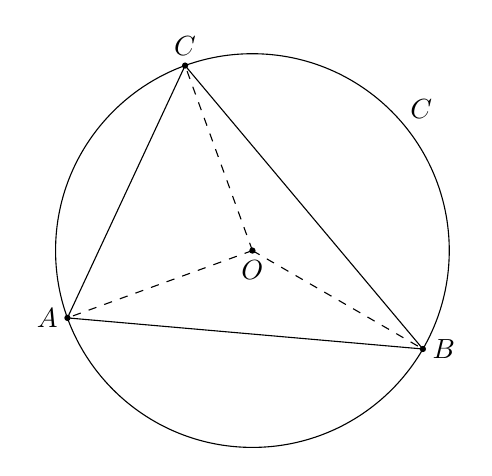
\begin{tikzpicture}[scale=1.0]

% parameters %{{{1

	\def\ang{200}
	\def\ngl{-30}
	\def\gle{110}

	\def\radius{2.5}

% coordinates %{{{1

	\coordinate (O) at (0,0);
	\coordinate (A) at (\ang:\radius);
	\coordinate (B) at (\ngl:\radius);
	\coordinate (C) at (\gle:\radius);

% points, dots, vertices %{{{1

	\fill (O) circle (0.4mm);
	\fill (A) circle (0.4mm);
	\fill (B) circle (0.4mm);
	\fill (C) circle (0.4mm);

% segments, sides %{{{1

	\draw (A) -- (B) -- (C) -- cycle;

	\draw[dashed] (O) -- (A);
	\draw[dashed] (O) -- (B);
	\draw[dashed] (O) -- (C);

% circles %{{{1

	\draw (O) circle (\radius);

% points, dots, vertices labels %{{{1

	\node[below] at (O) {$O$};
	\node[left] at (A) {$A$};
	\node[right] at (B) {$B$};
	\node[above] at (C) {$C$};

% segments, sides, lines marks %{{{1

	\tkzMarkSegments[mark=||, size=2pt](O,A)
	\tkzMarkSegments[mark=||, size=2pt](O,B)
	\tkzMarkSegments[mark=||, size=2pt](O,C)

% circle label %{{{1

	\node at (40:{\radius+0.3}) {$\mathscr{C}$};

% closing %{{{1

\end{tikzpicture}
\end{document}
